\documentclass[12pt,a4paper]{report}

\usepackage[T2A]{fontenc}
\usepackage[utf8]{inputenc}
\usepackage[bulgarian,english]{babel}
\usepackage{csquotes}
\usepackage[a4paper,margin=2.5cm]{geometry}
\usepackage{graphicx}
\usepackage{xcolor}
\usepackage{hyperref}
\usepackage{float}
\usepackage{booktabs}
\usepackage{longtable}
\usepackage{array}
\usepackage{enumitem}
\usepackage{listings}
\usepackage{caption}
\usepackage{setspace}
\usepackage{titlesec}
\usepackage{etoolbox}
\usepackage[nameinlink,noabbrev]{cleveref}

\AtBeginDocument{\selectlanguage{bulgarian}}

\addto\captionsbulgarian{
    \renewcommand{\contentsname}{Съдържание}
    \renewcommand{\chaptername}{Глава}
    \renewcommand{\bibname}{Литература}
    \renewcommand{\figurename}{Фигура}
    \renewcommand{\tablename}{Таблица}
    \renewcommand{\lstlistingname}{Код}
}

\hypersetup{
    colorlinks=true,
    linkcolor=blue,
    urlcolor=blue,
    citecolor=blue,
    pdftitle={CVAnalysisHub Documentation},
    plainpages=false
}

\crefname{chapter}{глава}{глави}
\Crefname{chapter}{Глава}{Глави}
\crefname{section}{раздел}{раздели}
\Crefname{section}{Раздел}{Раздели}
\crefname{subsection}{подраздел}{подраздели}
\Crefname{subsection}{Подраздел}{Подраздели}
\crefname{figure}{фигура}{фигури}
\Crefname{figure}{Фигура}{Фигури}
\crefname{table}{таблица}{таблици}
\Crefname{table}{Таблица}{Таблици}
\crefname{lstlisting}{код}{кодове}
\Crefname{lstlisting}{Код}{Кодове}

\raggedbottom
\emergencystretch=2em
\setstretch{1.15}
\setlength{\parskip}{0.4em}
\setlength{\parindent}{0pt}

\makeatletter
\patchcmd{\chapter}{\if@openright\cleardoublepage\else\clearpage\fi}{}{}{}
\makeatother
\pretocmd{\chapter}{\par\vspace{1.5\baselineskip}}{}{}

\titleformat{\chapter}[block]
  {\bfseries\Large}
  {\chaptername\ \thechapter}
  {0.8em}
  {\LARGE}
\titlespacing*{\chapter}{0pt}{1.2em}{0.8em}

\lstdefinestyle{csharpstyle}{
    language=[Sharp]C,
    basicstyle=\ttfamily\small,
    keywordstyle=\color{blue},
    commentstyle=\color{teal},
    stringstyle=\color{red!70!black},
    showstringspaces=false,
    breaklines=true,
    columns=fullflexible,
    keepspaces=true,
    frame=single,
    rulecolor=\color{black!20},
    backgroundcolor=\color{black!2},
    numbers=left,
    numberstyle=\scriptsize\color{black!45},
    xleftmargin=1.8em,
    framexleftmargin=1.2em,
    captionpos=b
}

\lstset{style=csharpstyle}

\newcommand{\projectname}{CVAnalysisHub}

\newcommand{\optionalfigure}[4][0.95\textwidth]{
    \begin{figure}[htbp]
        \centering
        \IfFileExists{#2}{
            \includegraphics[
                width=#1,
                height=0.58\textheight,
                keepaspectratio
            ]{#2}
        }{
            \fbox{
                \parbox[c][6cm][c]{0.86\textwidth}{
                    \centering
                    \textbf{Placeholder for figure}\\[0.6em]
                    File expected at: \texttt{#2}
                }
            }
        }
        \caption{#3}
        \label{#4}
    \end{figure}
}


\begin{document}
\selectlanguage{bulgarian}
\pagenumbering{gobble}

\begin{titlepage}
\thispagestyle{plain}

\noindent
\begin{minipage}{0.17\textwidth}
    \IfFileExists{figures/branding/3_TU_bg_n.png}{
        
\includegraphics[width=\linewidth]{figures/branding/3_TU_bg_n.png}
    }{
        \fbox{
            \parbox[c][3.5cm][c]{\linewidth}{
                \centering
                TU\\logo
            }
        }
    }
\end{minipage}%
\hspace{0.03\textwidth}%
\begin{minipage}{0.8\textwidth}
    \raggedright
    \large
    \textbf{ТЕХНИЧЕСКИ УНИВЕРСИТЕТ -- СОФИЯ}\\[-0.3ex]
    \rule{\linewidth}{0.2pt}\\[-0.6ex]
    \textbf{ФАКУЛТЕТ КОМПЮТЪРНИ СИСТЕМИ И ТЕХНОЛОГИИ}\\[0.2cm]
\end{minipage}

\vspace{3cm}

\begin{center}
    \textbf{\LARGE КУРСОВ ПРОЕКТ}\\[1cm]

    \normalsize
    Дисциплина: Програмни Среди\\[0.8cm]

    \textbf{Тема:}\\[0.3cm]
    \textbf{\projectname{} -- платформа за управление на видео анализи\\
    с компютърно зрение, Blazor, Avalonia и две СУБД}\\[2.8cm]
\end{center}

\vspace{0.8cm}

\begin{flushleft}
\textbf{Изготвил:}\\
Асен Пантелеев Попов\\
Фак. № 121223246\\
Група 38\\
III курс, КСИ\\
e-mail: \texttt{asepopov@tu-sofia.bg}
\end{flushleft}

\vspace{1.2cm}

\begin{flushleft}
\textbf{Преподавател:}\\
гл. ас. П. Маринов\\
\end{flushleft}

\vfill

\begin{center}
София, 2026 г.
\end{center}
\end{titlepage}

\cleardoublepage
\pagenumbering{roman}
\setcounter{page}{1}
\phantomsection
\tableofcontents
\cleardoublepage
\pagenumbering{arabic}
\setcounter{page}{1}

\chapter{Въведение}

\projectname{} представлява курсов проект, насочен към управление на видео анализи с помощта на компютърно зрение. Практическата идея на системата е потребителят да може да качва локални видеа, да създава задачи за анализ върху тях, да следи изпълнението на тези задачи и да преглежда резултатите от разпознаването на обекти. Темата е избрана така, че да бъде едновременно достатъчно практическа и достатъчно богата архитектурно, за да позволи смислена реализация на пълноценен софтуерен сценарий.

Проектът не е замислен като обикновен CRUD пример. Неговата цел е да демонстрира как в рамките на .NET екосистемата може да се изгради приложение с реален домейн, ясно разделение на отговорностите и преизползване на логика между няколко технологични слоя. В случая това преизползване се проявява в две направления. От една страна едни и същи споделени ViewModel-и обслужват два различни потребителски интерфейса. От друга страна едни и същи абстракции на модела и бизнес логиката работят с две различни системи за управление на бази данни.

Функционално системата обединява няколко последователни сценария. Първо се качва изходно видео, което се съхранява във файловото хранилище на приложението. След това върху него се създава задача за анализ. Тази задача се обработва асинхронно от фонов обработчик, който извиква избрания модул за инференция. При реалния сценарий с YoloDotNet се извличат подбрани кадри, върху тях се изпълнява разпознаване на обекти, резултатите се записват в базата данни и накрая се генерира анотирано изходно видео. Потребителят може да преглежда както историята от анализи, така и детайлите за конкретно изпълнение, включително откритите обекти и получения видео резултат.

Архитектурно проектът е реализиран така, че логиката на представяне да бъде максимално споделена, а специфичните за конкретната технология елементи да останат тънък слой върху общия приложен слой. Именно поради това структурата на проекта не е сведена до механични папки от тип \texttt{Views}, \texttt{ViewModels} и \texttt{Models}, а е организирана в по-реалистични слоеве: \texttt{Core}, \texttt{Application}, \texttt{Infrastructure}, \texttt{Web} и \texttt{Avalonia}. Тази организация позволява по-ясно разделение между домейн модела, приложната логика, инфраструктурните зависимости и визуализацията.

Настоящата документация има за цел да представи както крайния резултат, така и инженерните решения зад него. По-конкретно се разглеждат избраните технологии, условията за използването им, архитектурната организация на проекта, начинът на преизползване на ViewModel-и и на СУБД, преизползваемите механизми за филтриране и визуализация на списъци, както и примерни сценарии на работа. В края са обобщени и основните изводи от разработката, включително трудностите, които се наложи да бъдат преодолени.

Изходният код, README описанието и документацията на проекта са публикувани в GitHub репото \url{https://github.com/Apsie09/CV-Analysis-Hub}.

\chapter{Използвани технологии}

\section{View технологии}

\subsection{Blazor}

Blazor е избран като уеб технология в проекта, тъй като позволява изграждане на интерактивен потребителски интерфейс изцяло в .NET среда, без необходимост от отделен приложен слой на JavaScript. За конкретната разработка това се оказва особено удобно, защото споделените ViewModel-и могат да бъдат инжектирани директно в компонентите и използвани като основен източник на състоянието на интерфейса. Освен това Blazor е много подходящ за изграждане на преизползваеми елементи на интерфейса, каквито в проекта са панелът за филтриране и компонентът за визуализация на списъци.

Blazor е полезен не само като технология за потребителски интерфейс, а и като добра среда за изграждане на автоматизирано генериран потребителски интерфейс върху общи приложни абстракции. Компонентният модел на Blazor улеснява изграждането на повторно използваеми визуални елементи, които работят върху метаданни и ViewModel-и, а не върху конкретни класове от модела. Това го прави подходящ избор за филтри, таблици и детайлни изгледи, които се повтарят в различни части на приложението.

\subsection{AvaloniaUI}

Avalonia е избрана като настолна технология, защото предоставя XAML, модел на обвързване и команди, близък до класически MVVM инструменти като WPF, но без да бъде ограничена само до Windows. Това е важен практически аргумент, тъй като проектът се разработва и тества под Linux. В тази среда Avalonia позволява реална настолна реализация със сравнително тънък code-behind и естествено обвързване със споделен ViewModel слой.

В контекста на настоящия проект Avalonia е използвана като пълноценен настолен клиент, а не само като минимална визуална обвивка. Настолният клиент реално поддържа обзорни метрики, преглед на видео библиотеката, качване на видеа, стартиране на анализи, разглеждане на историята от изпълнения и визуализация на резултатите. По този начин се демонстрира, че споделените приложни ViewModel-и могат да обслужват втори интерфейс с реална функционалност.

\section{Системи за управление на бази данни}

\subsection{SQLite}

SQLite е подходяща за локална разработка и за демонстрационни сценарии, тъй като не изисква отделен сървър и работи чрез един файл. Това я прави удобна за бързо стартиране на приложението, за преносима демонстрационна конфигурация и за ситуации, в които е важно системата да може да бъде показана без допълнителна инсталация на сървър за база данни. В рамките на проекта SQLite е естествен избор за лек режим на работа и за лесна повторяемост при локално тестване.

Същевременно SQLite има и ограничения. Тя не отразява напълно типична експлоатационна среда и не е най-подходящият избор за по-сериозен многопотребителски сценарий. Именно поради това в проекта е включена и PostgreSQL, така че слоят за съхранение да не бъде обвързан само с една удобна за разработка технология.

\subsection{PostgreSQL}

PostgreSQL е избрана като втора СУБД, защото е значително по-близка до реална сървърна среда. Тя предоставя по-богата екосистема, по-реалистичен модел на внедряване и добра интеграция с EF Core чрез Npgsql. В контекста на проекта PostgreSQL показва, че една и съща приложна и бизнес логика може да работи върху различни доставчици без дублиране на код.

Най-същественото тук е, че проектът не поддържа две бази чрез два отделни service слоя. Вместо това същият \texttt{AppDbContext}, същите инфраструктурни услуги и същите приложни ViewModel-и работят и с SQLite, и с PostgreSQL. Разликата се свежда до конфигурационен избор на доставчик, а не до паралелни имплементации със същата логика.

\section{Други използвани технологии}

\subsection{Entity Framework Core}

Entity Framework Core е основата на слоя за съхранение. Чрез него проектът получава общ модел на данните, общ механизъм за заявки и възможност за превключване между SQLite и PostgreSQL. За конкретната разработка EF Core е ценен и с това, че позволява приложната логика да остане сравнително чиста и независима от конкретния доставчик на база данни, докато инфраструктурният слой поема конфигурацията и реалната интеграция с базата.

\subsection{YoloDotNet, ONNX Runtime и ffmpeg}

Важна особеност на проекта е, че частта за видео анализ не е оставена на ниво симулация. Вместо фиктивни записи за разпознати обекти е реализирана работеща последователност с \texttt{YoloDotNet}, ONNX модел и \texttt{ffmpeg}. \texttt{ffmpeg} се използва за извличане на подбрани кадри и за рендериране на анотирано изходно видео, а YoloDotNet изпълнява разпознаване на обекти върху тези кадри. Именно тази комбинация превръща приложението от обикновен административен интерфейс в система с реална аналитична функционалност.

Официалният проект на YoloDotNet го представя като модулна .NET библиотека за YOLO инференция, която стъпва върху ONNX Runtime и е насочена към предвидимо и производително изпълнение без Python среда за изпълнение и без тежки външни библиотеки за компютърно зрение \cite{yolodotnet}. Тази идея съответства много добре на целите на настоящия проект, защото \projectname{} също се стреми към изцяло .NET реализация, която да бъде лесна за демонстрация и достатъчно компактна за учебна среда.

Разпознаването на обекти представлява задача от компютърното зрение, при която системата трябва едновременно да определи какъв обект присъства в изображението и къде точно се намира той. За разлика от обикновената класификация, тук не е достатъчно да се каже, че в кадъра има човек или автомобил. Необходимо е и локализиране на всеки обект чрез ограничителна рамка, както и оценка на увереността на модела. Именно този тип резултат се съхранява в \projectname{} под формата на етикет, увереност и координати на ограничителната рамка.

\optionalfigure[0.78\textwidth]{figures/branding/object_detection_example.png}{Пример за резултат от разпознаване на обекти с bounding boxes}{fig:object-detection-example}

В основата на много modern computer vision модели стоят конволюционните невронни мрежи. Тяхната идея е, че чрез конволюционни филтри могат да се извличат локални визуални признаци като контури, текстури и по-сложни пространствени структури. С нарастване на дълбочината на мрежата тези признаци стават все по-абстрактни и подходящи за разпознаване на цели обекти. Макар съвременните YOLO архитектури да съдържат и допълнителни оптимизации, връзката им с CNN подхода остава фундаментална, защото те също използват learnable feature extraction върху изображението, за да достигнат до финално предсказване.

\optionalfigure[0.72\textwidth]{figures/branding/CNN.png}{Схематично представяне на конволюционна невронна мрежа}{fig:cnn-overview}

YOLO, съкратено от \textit{You Only Look Once}, е семейство от едностъпкови модели за разпознаване на обекти. Основната идея е, че вместо да се правят отделни етапи за генериране на предложения за региони и последваща класификация, моделът обработва изображението в един общ проход за инференция и директно предсказва класове и ограничителни рамки. Това го прави особено подходящ за приложения, в които е важен балансът между точност и скорост, например обработка на видео и почти реално време.

\optionalfigure[0.82\textwidth]{figures/branding/Yolo_Algorithm.png}{Схема на общата идея зад YOLO алгоритмите}{fig:yolo-algorithm}

В проекта е избрана серията YOLOv8. Причината не е единствено популярността на модела, а добрият практически баланс между зрялост на екосистемата, стабилна документация, лесен export към ONNX и широка поддръжка в инструменти като Ultralytics и YoloDotNet. Официалната екосистема на Ultralytics представя YOLOv8 като state-of-the-art поколение, създадено за задачи като detect, segment, classify и pose, с няколко размерни варианта, които позволяват избор според конкретния хардуер и натоварване \cite{ultralyticsyolov8, ultralyticsmodels}.

По-конкретно в \projectname{} се използва \texttt{yolov8n.onnx}, тоест nano вариантът на YOLOv8. Този избор е напълно логичен за учебен проект, който трябва да работи надеждно на стандартна машина и в настолно приложение с CPU доставчик за изпълнение. Според публикуваните от Ultralytics сравнения nano моделът е най-малкият вариант по брой параметри и изчислителна сложност, като същевременно остава практически полезен за реални задачи по детекция \cite{ultralyticsmodels}. С други думи, избраният модел не максимизира абсолютната точност, а търси добър инженерeн компромис между време за инференция, използвана памет и достатъчно добри резултати за демонстрация върху видео.

Този избор на технологии носи и практическа стойност за документацията. Проектът показва не само UI и работа с база данни, а и интеграция с външен инструмент и с библиотека за машинно зрение. Следователно той обхваща по-широк спектър от инженерни задачи, отколкото стандартен учебен пример.

\chapter{Какво беше необходимо, за да работят технологиите}

Една от важните части на заданието е да се опише не само видимата функционалност, но и интеграционната работа, без която крайният резултат не би бил възможен. В настоящия проект именно тази невидима на пръв поглед работа се оказа съществена. Архитектурно кодът можеше да изглежда правилен още в ранна фаза, но реалното съгласуване между уеб и настолния клиент, между двете бази данни и между обработката на видео и потребителския интерфейс изискваше допълнителни решения.

\section{Съгласуване на конфигурацията}

За да могат двата клиента да показват еднакви данни и да работят последователно, се оказа необходимо и двата да сочат към една и съща конфигурационна среда. Това включва не само избора на \texttt{Persistence:Provider}, но и еднакъв низ за свързване, еднакво файлово хранилище, еднакъв път към ONNX модела и еднаква конфигурация за \texttt{ffmpeg}. Без това приложението би изглеждало функционално, но двата клиента биха могли да показват различни данни и така да създадат погрешно впечатление за архитектурно разминаване.

Тази особеност е важна и от гледна точка на защитата. Изискването за две UI технологии не означава две независими програми, а две визуализации върху споделена приложна логика. Аналогично, изискването за две СУБД не означава два отделни проекта, а един модел и един бизнес слой, който работи и с двата доставчика. Следователно правилната конфигурация е част от архитектурната демонстрация, а не просто техническа подробност.

\section{Стартиране на настолния клиент и фонови услуги}

При Avalonia се появи специфичен проблем. Ако настолното приложение използва само ръчно конструиран \texttt{ServiceCollection}, фонова услуга като обработчика на анализи няма да бъде стартирана по същия начин, както в уеб приложението. За да се избегне това разминаване, Avalonia клиентът беше свързан към \texttt{IHost}. По този начин настолното приложение започна да използва същия модел за инжектиране на зависимости, фонови услуги и конфигурация, който вече съществуваше в уеб слоя.

Това решение се оказа ключово, защото позволи \texttt{QueuedAnalysisBackgroundService} да работи и в настолната среда и доближи стартирането на двата клиента. Така Avalonia приложението се превърна в реално функционален интерфейс, а не само във формално доказателство за втора технология.

\section{Медийна последователност и обработка на видео}

Друг важен слой от работа беше свързан с реалната обработка на видео. За да не остане приложението на ниво административен интерфейс с фиктивни резултати, беше необходимо качените файлове действително да се записват във файлово хранилище, от тях да се извличат кадри чрез \texttt{ffmpeg}, тези кадри да се подават към YOLO модела и накрая да се генерира анотирано изходно видео.

Тази интеграция не е видима директно от структурата на решението, но е сърцевината на функционалността. Тя обвързва файловата система, външния инструмент за обработка на видео, модула за инференция и слоя за съхранение в един последователен процес. Без такава реализация приложението би имало добра архитектура, но не би показвало реален аналитичен резултат.

\section{Работа под Linux и локална среда}

Фактът, че разработката и тестването се извършват под Linux, постави и няколко допълнителни изисквания. Наложи се да бъде конфигуриран коректен път към \texttt{/usr/bin/ffmpeg}, да се вземе предвид поведението на локалните HTTPS сертификати в браузъра и да се намери подходящ настолен подход за визуализация на видео без въвеждане на тежка зависимост за вградено възпроизвеждане. В резултат настолният клиент комбинира предварителни кадри и отваряне на оригиналното или обработеното видео чрез системния видео плейър.

Тук ясно се вижда разликата между това кодът да е написан и това приложението да е действително работещо в реална среда. Именно тези интеграционни аспекти често не се забелязват в крайния продукт, но представляват съществена част от извършената инженерна работа.

\chapter{Архитектура}

\section{Общ архитектурен модел}

Проектът използва слоеста архитектура с MVVM на ниво представяне. Това означава, че ролите на \textit{View}, \textit{ViewModel} и \textit{Model} са налице, но не са материализирани като три механични папки в един и същ проект. Вместо това те са разпределени по слоеве според отговорностите си. View частта се реализира от Blazor компонентите и Avalonia XAML екраните. ViewModel частта е концентрирана основно в приложния слой чрез споделени ViewModel-и, а при настолния клиент има допълнителен координиращ ViewModel за специфично поведение на интерфейса. Model частта е по-широко понятие и включва домейн обекти, DTO-та, заявки, service contract-и и инфраструктурни услуги.

Този подход е по-подходящ за реален .NET проект, отколкото просто физическо групиране по три папки, защото позволява домейн логиката да остане изолирана от грижите на потребителския интерфейс, а споделената приложна логика да бъде преизползвана от повече от една View технология. Диаграмата на \cref{fig:mvvm-mapping} показва точно това съответствие между MVVM ролите и конкретните части на проекта, докато \cref{fig:architecture-overview} представя по-общия слоест изглед на системата.

\optionalfigure{figures/generated/mvvm-mapping.png}{MVVM картографиране в проекта: кои части са View, ViewModel и Model}{fig:mvvm-mapping}

\optionalfigure{figures/generated/architecture-overview.png}{Обща архитектурна диаграма на проекта}{fig:architecture-overview}

Към собствените диаграми в документацията може да се добави и външен архитектурен поглед върху репото, генериран чрез \href{https://github.com/CodeBoarding/CodeBoarding}{CodeBoarding}. Тази визуализация не замества ръчния архитектурен анализ, а служи като бърза карта за ориентация в структурата на проекта и в зависимостите между основните му слоеве.

\optionalfigure[0.46\textwidth]{figures/screenshots/Codeboarding_output.png}{Външно архитектурно обобщение на \projectname, получено чрез CodeBoarding}{fig:codeboarding-output}

\section{Слоеве на системата}

\subsection{\texttt{CVAnalysisHub.Core}}

\texttt{CVAnalysisHub.Core} е домейн слоят на проекта. В него се намират основните бизнес обекти \texttt{Video}, \texttt{AnalysisRun} и \texttt{DetectionResult}. Тези типове описват бизнес данните и връзките между тях, без да зависят нито от конкретна технология за потребителски интерфейс, нито от конкретен доставчик на база данни. Така те изпълняват ролята на стабилно ядро, върху което се изграждат останалите слоеве.

\subsection{\texttt{CVAnalysisHub.Application}}

\texttt{CVAnalysisHub.Application} съдържа приложни абстракции и споделена логика на представяне. В този слой се намират DTO-тата, моделите на заявки, service contract-ите, споделените ViewModel-и, както и преизползваемите абстракции за филтри и за списъци от обекти. Именно тук е реализирана същинската идея за преизползване на ViewModel-и от различни View технологии. Вместо всяка технология да получи собствен набор от класове със сходна функционалност, и уеб, и Avalonia клиентът използват един и същ приложен слой.

\subsection{\texttt{CVAnalysisHub.Infrastructure}}

Infrastructure слоят съдържа конкретните имплементации на услугите за съхранение, медийна обработка и анализ. Тук се намират EF Core контекстът, service класовете, конфигурацията на доставчика на база данни, файловото хранилище, логиката за обработка на видео, модулите за инференция и фоновият обработчик за чакащите анализи. Това е слоят, който осигурява взаимодействието с външните технологии, без да пренася техните зависимости към домейн и приложния слой.

\subsection{\texttt{CVAnalysisHub.Web} и \texttt{CVAnalysisHub.Avalonia}}

\texttt{CVAnalysisHub.Web} представлява уеб слоя на представяне и съдържа Blazor интерфейса, преизползваеми Razor компоненти и composition root-а за уеб изпълнение. \texttt{CVAnalysisHub.Avalonia} е настолният слой на представяне и съдържа Avalonia XAML View-та, както и минимален специфичен за технологията слой за координация на настолния интерфейс. Същественото тук е, че тези два проекта изпълняват различни View роли, но не дублират основната логика на представяне, а я използват от общия приложен слой.

\subsection{Външно архитектурно резюме}

CodeBoarding дава на разработчици и coding agents визуална карта на дадена кодова база. Инструментът комбинира статичен анализ с LLM reasoning, за да генерира архитектурни диаграми, документация на ниво компоненти и навигируеми изходи, които могат да се използват в IDE, CI процеси и документация \cite{codeboarding}. В \cref{fig:codeboarding-output} той е използван като допълнителен поглед към структурата на \projectname, а не като заместител на ръчния архитектурен анализ. CodeBoarding е стартъп, започнат от Иван Милев, който е възпитаник на Технически университет -- София, продължава обучението си с магистратура в ETH Zurich и към момента развива проекта в Силициевата долина.

\begin{description}
\item[Application Logic \& State] CodeBoarding обобщава този слой като мястото, в което се оркестрира бизнес логиката и се управлява състоянието на интерфейса чрез shared ViewModel-и и service абстракции. Това съответства пряко на ролята на \texttt{CVAnalysisHub.Application}.
\item[Background Analysis Processor] Тук инструментът разпознава жизнения цикъл на задачите за анализ и координацията между медийния двигател и persistence слоя чрез фонов обработчик. Това отговаря на hosted service слоя за обработка на чакащи анализи и на свързаните processing услуги.
\item[Web Presentation Layer] Уеб клиентът е разпознат като Blazor слой на представяне, който управлява потребителските взаимодействия и браузърното изпълнение. Това е \texttt{CVAnalysisHub.Web}.
\item[Desktop Presentation Layer] Настолният клиент е разпознат като Avalonia слой на представяне, който споделя приложната логика с уеб клиента чрез общите ViewModel-и. Това е \texttt{CVAnalysisHub.Avalonia}.
\item[Computer Vision \& Media Engine] CodeBoarding отделя тежката медийна обработка, извличането на кадри и ML детекцията чрез YOLO и ONNX runtime. Това съвпада с \texttt{VideoProcessingService} и \texttt{YoloDotNetAnalysisInferenceEngine}.
\item[Data Persistence \& Infrastructure] Този слой е описан като отговорен за съхранението и извличането на данни чрез Entity Framework Core и за реализацията на service contract-ите към SQLite или PostgreSQL. Това е ролята на \texttt{CVAnalysisHub.Infrastructure}.
\item[Domain Model] Домейн моделът е разпознат като ядро от бизнес обекти, описващи основните понятия в системата, като \texttt{Video}, \texttt{AnalysisRun} и \texttt{DetectionResult}. Това съответства на \texttt{CVAnalysisHub.Core}.
\end{description}

\section{Модел на базата данни}

Моделът на съхранение е умишлено компактен. Той не е прекалено сложен, защото проектът няма нужда от голям брой таблици, а от ясна структура, която поддържа основния бизнес сценарий. Моделът е достатъчно богат, за да реализира реален работен процес за видео анализ, и в същото време остава достатъчно малък, за да бъде лесен за обяснение и демонстрация.

Схемата съдържа три основни таблици. Таблицата \texttt{Video} описва качените видеа и пази връзка към файловото хранилище. Таблицата \texttt{AnalysisRun} представя конкретно изпълнение на анализ върху дадено видео и пази информация за модела, времето на изпълнение, статуса, броя открити обекти и изходния видео резултат. Таблицата \texttt{DetectionResult} пази единичните детекции за конкретно изпълнение, включително номер на кадър, етикет, увереност и координати на ограничителната рамка. По този начин едно видео може да има множество изпълнения на анализ, а всяко изпълнение може да съдържа множество резултати от детекция.

\optionalfigure{figures/generated/db-schema.png}{ER диаграма на основните таблици в проекта}{fig:db-schema}

\section{Последователност на анализа}

Една от важните архитектурни характеристики на проекта е, че последователността на анализа не е реализирана като директно синхронно действие от слоя на потребителския интерфейс. Вместо това процесът е разделен на ясни етапи. Първо потребителят качва видео и създава задача за анализ. След това се създава \texttt{AnalysisRun} със статус \texttt{Queued}. Фоновият обработчик периодично проверява за чакащи задачи, избира следващата и я премества в състояние \texttt{Processing}. Източникът се подава към избрания модул за инференция, който извлича кадри, изпълнява детекция, създава резултатите и накрая генерира анотирано изходно видео. В зависимост от изхода статусът се променя на \texttt{Completed} или \texttt{Failed}.

Този модел прави системата по-близка до реален работен процес, отколкото до демонстрационен сценарий само за настолен клиент. Освен това той отделя потребителския интерфейс от тежката обработка и позволява по-чиста организация на отговорностите между слоя на представяне, приложния слой и инфраструктурния слой.

\optionalfigure{figures/generated/analysis-flow.png}{Диаграма на анализа на видео в проекта}{fig:analysis-flow}

\chapter{Описание на реализацията}

\section{Разпределение на типовете по слоеве}

За да бъде архитектурата ясна и лесна за поддръжка, типовете в проекта са разпределени по слоеве според тяхната функция. В домейн слоя се намират основните обектни типове, които описват същинските бизнес обекти: видео, анализ и резултат от детекция. Тези класове не познават конкретна технология за потребителски интерфейс, нито начин на съхранение, което позволява да служат като стабилен модел на системата.

Приложният слой съдържа класовете, които оформят интерфейса между домейна и технологията за представяне. Тук се намират DTO-тата, моделите на заявки, service contract-ите и споделените ViewModel-и като \texttt{HomeViewModel}, \texttt{VideoListViewModel}, \texttt{CreateVideoViewModel}, \texttt{AnalysisRunListViewModel}, \texttt{CreateAnalysisRunViewModel} и \texttt{AnalysisRunDetailsViewModel}. В същия слой са разположени и преизползваемите абстракции за филтри и за списъци от обекти, които позволяват една и съща логика да се прилага върху различни екрани.

Infrastructure слоят съдържа реалните имплементации, върху които стъпва приложението: \texttt{AppDbContext}, EF Core service класовете, услугите за съхранение на файлове, логиката за обработка на видео, фоновата услуга и модулите за инференция. Така проектът остава ясно структуриран: приложният слой описва какво трябва да може системата, а инфраструктурният слой реализира как точно става това.

\section{Организация на преизползването на ViewModel-и}

Изискването за едни и същи ViewModel-и в две различни View технологии е едно от най-съществените за проекта. Вместо две паралелни дървета от класове със сходна функционалност, едното за уеб, а другото за настолен интерфейс, споделените ViewModel-и се намират в \texttt{CVAnalysisHub.Application} и се използват и от двата клиента.

Това преизползване е приложено в основните функционални сценарии на приложението. Обзорните метрики, списъците от видеа и анализи, филтрите, процесът на качване, процесът по създаване на анализ и детайлният преглед на избран analysis run са реализирани чрез споделени приложни ViewModel-и. Avalonia има собствен \texttt{MainWindowViewModel}, но неговата роля не е да дублира бизнес функционалността, а да координира специфичното за настолния клиент състояние на интерфейса върху тези споделени ViewModel-и, например предварителни кадри и действия за отваряне на изходното и обработеното видео.

\section{Организация на преизползването за двете СУБД}

Поддръжката на две СУБД е реализирана така, че да не се нарушава идеята за общ модел и обща бизнес логика. Не съществува отделен service слой за SQLite и отделен service слой за PostgreSQL. Вместо това изборът на доставчик се извършва конфигурационно в инфраструктурния слой. Там, въз основа на стойността на \texttt{Persistence:Provider}, се избира дали EF Core да използва \texttt{UseSqlite} или \texttt{UseNpgsql}.

Тази организация избягва дублиране на една и съща логика за всяка СУБД. В текущия проект домейн и приложният слой не се интересуват кой точно доставчик стои отдолу. За тях услугата за съхранение е една и съща по поведение, което позволява системата да бъде стартирана и с SQLite, и с PostgreSQL без промяна във ViewModel-ите и без пренаписване на бизнес логиката.

\section{Организация на преизползваемите UI механизми}

Преизползваемата функционалност за филтриране е реализирана чрез общ модел на метаданни за полетата на филтрите. Всеки екран с търсене описва полетата си чрез надпис, описание, тип на входа и подсказващи текстове. Въз основа на тези метаданни преизползваемият визуализатор избира подходяща контрола, например текстово поле, падащ списък, числов интервал или интервал от дати. Въведените стойности не остават на ниво интерфейс, а се трансформират в типизирана заявка за търсене, която се използва от слоя за съхранение за изграждане на заявка към базата данни. Най-важното е, че тази функционалност не е написана за една конкретна таблица, а е демонстрирана върху два различни модела: \texttt{Videos} и \texttt{AnalysisRuns}.

По сходен начин е реализирана и преизползваемата функционалност за визуализиране на списъци от обекти. На преизползваемия list ViewModel се подава списък от DTO обекти, конфигурират се видимите колони и при избор на ред може да се върне целият избран обект, независимо кои свойства са били визуализирани. Визуализацията може да се изчиства и зарежда отново с нов списък. Същият механизъм е приложен върху \texttt{Videos} и \texttt{AnalysisRuns}, което показва, че таблицата и selection логиката не са обвързани с един конкретен модел.

\section{Ключови решения в кода}

Едно от най-важните архитектурни решения е превключването между SQLite и PostgreSQL. В проекта това не е реализирано чрез два различни слоя за съхранение, а чрез централизирана конфигурация в инфраструктурния слой. Така приложната логика остава една и съща, а конкретният доставчик се избира в стартовата конфигурация.

\lstinputlisting[
    firstline=16,
    lastline=83,
    caption={Откъс от \texttt{DependencyInjection.cs}, който избира SQLite или PostgreSQL},
    label={code:provider-switch}
]{../CVAnalysisHub.Infrastructure/DependencyInjection.cs}

Кодът от \cref{code:provider-switch} показва две важни идеи. Първо, низът за свързване се определя спрямо стойността на \texttt{Persistence:Provider}, а не е фиксиран в приложния слой. Второ, изборът между \texttt{UseSqlite} и \texttt{UseNpgsql} е концентриран на едно място. Именно това прави възможно изпълнението на едно и също приложение върху две СУБД без дублиране на бизнес логика.

Втората съществена част е слоят със споделени ViewModel-и. Следният откъс показва, че \texttt{VideoListViewModel} не е специфичен нито за Blazor, нито за Avalonia. Той комбинира споделени филтри, преизползваем списък от обекти и зареждане на данни през service contract, което му позволява да бъде използван от двата интерфейса.

\lstinputlisting[
    firstline=6,
    lastline=84,
    caption={Откъс от \texttt{VideoListViewModel.cs} със shared list и filter логика},
    label={code:video-list-vm}
]{../CVAnalysisHub.Application/Videos/VideoListViewModel.cs}

Откъсът от \cref{code:video-list-vm} показва как преизползваемата функционалност е капсулирана на ниво ViewModel, а не само на ниво визуален компонент. Списъкът от видеа, активните филтри, зареждането на резултатите и изборът на ред са организирани в една споделена приложна абстракция, която после се визуализира по различен начин от Blazor и Avalonia.

Преизползването не остава само в ViewModel слоя. \cref{code:object-list-table} показва и кратък реален пример от Blazor компонента за визуализация на списъци. Компонентът е generic, работи с \texttt{ObjectListViewModel<TItem>}, взима видимите колони от ViewModel-а и връща избрания ред като пълен обект, а не само като стойности от таблицата.

\lstinputlisting[
    firstline=1,
    lastline=60,
    caption={Откъс от \texttt{ObjectListTable.razor} като generic reusable list компонент},
    label={code:object-list-table}
]{../CVAnalysisHub.Web/Components/Shared/ObjectListTable.razor}

Следващият кратък откъс показва как задачите за анализ се отделят от потребителския интерфейс. \texttt{QueuedAnalysisBackgroundService} периодично търси чакащ анализ, създава scope за инфраструктурните услуги и делегира реалната обработка към \texttt{IAnalysisRunProcessor}. Така UI слоят създава задача, но не носи тежестта на самата обработка.

\lstinputlisting[
    firstline=8,
    lastline=35,
    caption={Откъс от \texttt{QueuedAnalysisBackgroundService.cs} за обработка на чакащи анализи},
    label={code:queued-worker}
]{../CVAnalysisHub.Infrastructure/AnalysisRuns/QueuedAnalysisBackgroundService.cs}

Последният ключов фрагмент е свързан с реалната последователност на инференцията. По-долу е показан съкратен откъс от модула, който интегрира YoloDotNet, извличането на кадри и генерирането на анотирано видео.

\lstinputlisting[
    firstline=23,
    lastline=98,
    caption={Откъс от \texttt{YoloDotNetAnalysisInferenceEngine.cs} с основния inference pipeline},
    label={code:yolo-engine}
]{../CVAnalysisHub.Infrastructure/AnalysisRuns/YoloDotNetAnalysisInferenceEngine.cs}

\cref{code:yolo-engine} показва, че анализът не се свежда до запис на фиктивни стойности в базата. Първо се валидира изходното видео и се създава временна работна директория. След това кадрите се извличат чрез \texttt{VideoProcessingService}, върху всеки кадър се извиква \texttt{RunObjectDetection}, резултатите се преобразуват в удобна за домейна структура, рисуват се ограничителни рамки и накрая се рендерира изходно анотирано видео. Така аналитичната стойност на проекта е свързана с изпълним цялостен процес, а не само с визуализация на предварително подготвени данни.

При Avalonia клиента визуализацията на медийното съдържание е реализирана чрез предварителни кадри и отваряне на оригиналното или обработеното видео със системния видео плейър. Така настолното приложение използва съществуващата \texttt{ffmpeg} последователност, без да въвежда тежка вградена зависимост за възпроизвеждане на видео.

\section{Трудности и преодолени проблеми}

В процеса на реализация възникнаха няколко трудности, които оказаха влияние върху стабилността и завършеността на приложението. Сред тях бяха синхронизацията между Web и Avalonia при различни доставчици и различно файлово хранилище, логиката по стартиране на настолния клиент и фоновите услуги, проблеми с темата и контраста в Avalonia под Linux, поведението на локалния HTTPS сертификат за разработка в браузъра и необходимостта ясно да се разграничат статусът на видеото и статусът на анализа в интерфейса.

Един от по-полезните практически изводи беше, че архитектурно правилният код сам по себе си не е достатъчен за завършено приложение. Необходимо е системата да бъде не само правилно структурирана, но и стабилна, разбираема и без подвеждащи състояния на интерфейса. Точно поради тази причина в по-късните етапи беше обърнато внимание и на удобството за работа с Avalonia клиента, така че той да бъде реално използваем интерфейс.

\chapter{Примери за използване}

\section{Пример за завършен анализ}

Най-естественият начин за използване на системата започва с качване на локално видео. Потребителят избира файл от файловата система, приложението го записва във файловото хранилище и създава съответен запис в таблицата \texttt{Videos}. От този момент нататък видеото става част от общата библиотека и може да бъде използвано като източник за нов анализ. Ако двата клиента работят върху една и съща конфигурация, записът става видим и в уеб, и в настолния интерфейс.

След като съществува качено видео, може да се създаде нов \texttt{AnalysisRun}. От гледна точка на потребителя това е кратко действие от интерфейса, но вътрешно то създава задача, която по-късно се поема от фоновия обработчик. Така потребителското действие се отделя от тежката аналитична обработка и системата остава отзивчива дори при по-дълги операции. След приключване на анализа в базата се записват статусът, резултатите от детекцията и обработеното видео.

След завършване на анализа потребителят може да прегледа подробностите за конкретно изпълнение. Тук системата показва използвания модел, броя на разпознатите обекти, обобщение по етикети, оригиналното видео, анотираното изходно видео и таблица с отделните detection results. По този начин приложението демонстрира завършен сценарий от качване на видео до преглед на финален резултат.

\begin{table}[htbp]
\centering
\begin{tabular}{ll}
\toprule
Показател & Стойност \\
\midrule
Изходно видео & \texttt{crowd.mp4} \\
Използван модел & \texttt{yolov8n.onnx} \\
Статус на анализа & \texttt{Completed} \\
Общо открити обекти & 424 \\
Основен клас & \texttt{person} -- 409 разпознавания \\
Други класове & \texttt{bird} -- 6, \texttt{dog} -- 5, \texttt{handbag} -- 2 \\
Допълнителни класове & \texttt{skis} -- 1, \texttt{suitcase} -- 1 \\
\bottomrule
\end{tabular}
\caption{Примерни стойности от завършен анализ на видео \texttt{crowd.mp4}}
\label{tab:crowd-analysis-results}
\end{table}

\cref{tab:crowd-analysis-results} показва реален резултат от изпълнение на анализа. В този пример системата разпознава голям брой хора в кадрите, което съответства на съдържанието на видеото. Същите данни се визуализират както в Blazor клиента, така и в Avalonia клиента, когато двете приложения използват една и съща база данни и едно и също файлово хранилище.

\begin{lstlisting}[caption={Съкратен лог от изпълнението и обновяването на анализа}, label={code:analysis-demo-log}, language={}]
Video uploaded: crowd.mp4
Analysis run created with model: yolov8n.onnx
Run status: Queued -> Processing -> Completed
Output video and detections are ready
Objects detected: 424
Top labels: person=409, bird=6, dog=5, handbag=2
\end{lstlisting}

Логът от \cref{code:analysis-demo-log} не е пълен системен журнал, а съкратено представяне на съществените състояния в процеса на обработка. Те показват преминаването от качено видео към чакаща задача, последваща обработка, завършен анализ и записани резултати. Така примерът описва реален процес на обработка, а не визуализация на статични примерни данни.

\section{Екрани за демонстрация}

Екраните в тази секция показват завършения сценарий в двата потребителски интерфейса и илюстрират, че резултатите от анализа се четат от общия приложен слой. Blazor изгледът представя най-пълната визуализация на анализа, докато Avalonia изгледът използва същите данни и същите ViewModel-и в настолен клиент.

\IfFileExists{figures/screenshots/blazor-analysis-details_1.png}{
    \begin{figure}[htbp]
        \centering
        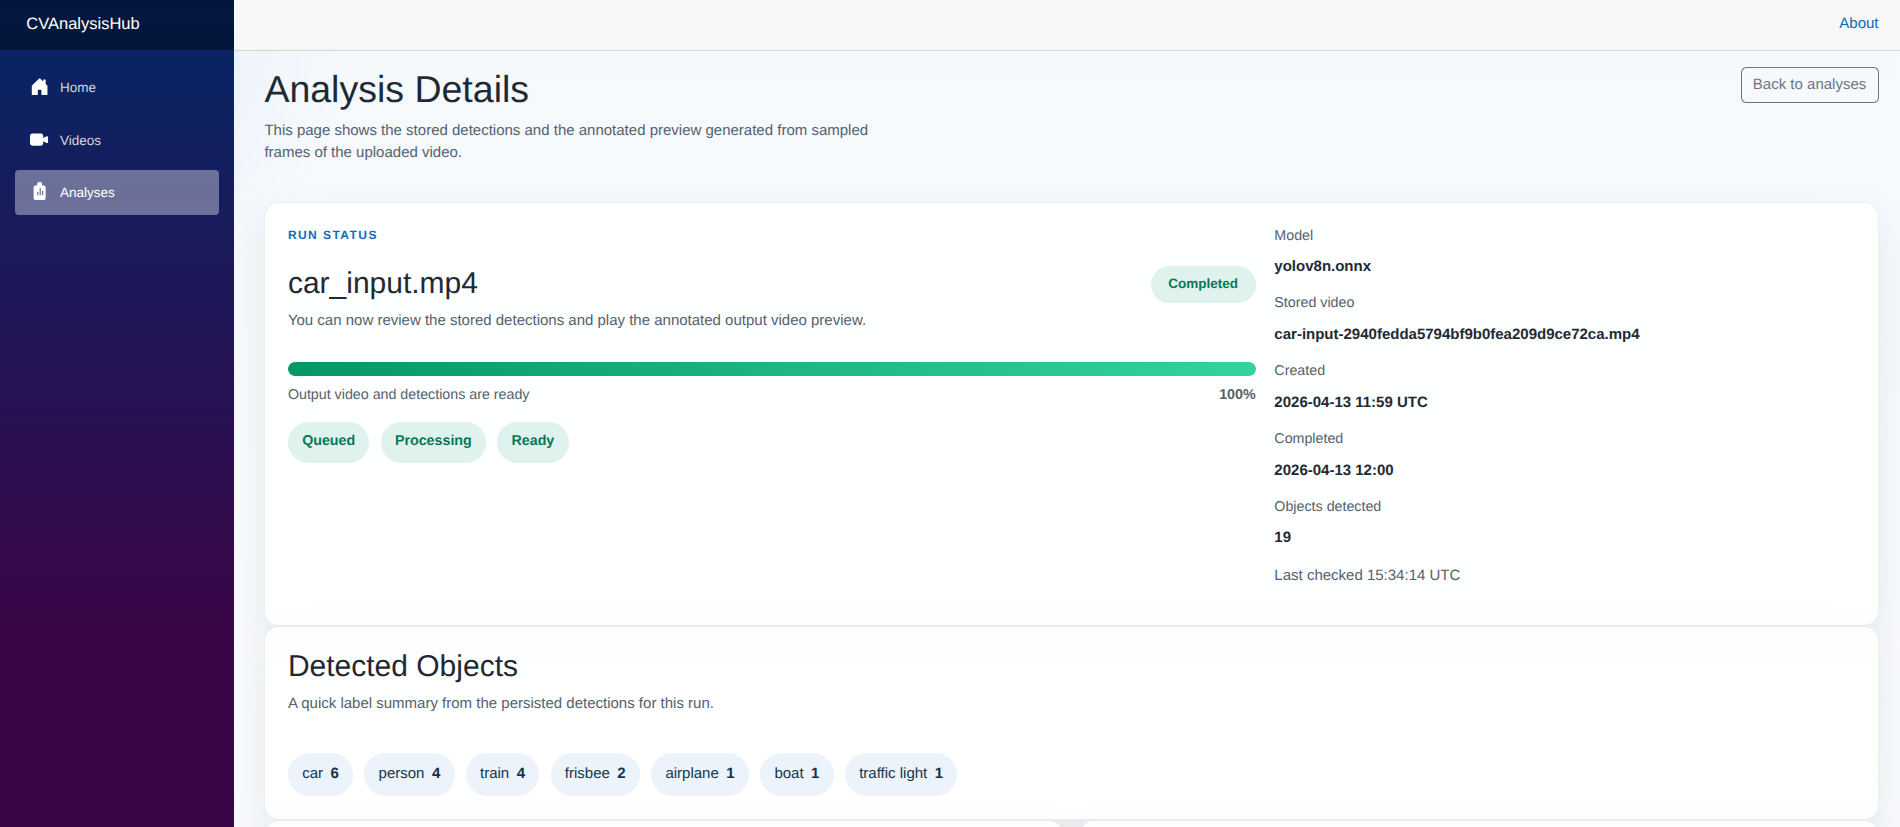
\includegraphics[width=0.95\textwidth,height=0.58\textheight,keepaspectratio]{figures/screenshots/blazor-analysis-details_1.png}
        \caption{Blazor интерфейс с подробности за завършен анализ, обобщение на разпознатите обекти и видео визуализация}
        \label{fig:blazor-analysis-details-overview}
    \end{figure}
}{}

\IfFileExists{figures/screenshots/blazor-analysis-details_2.png}{
    \begin{figure}[htbp]
        \centering
        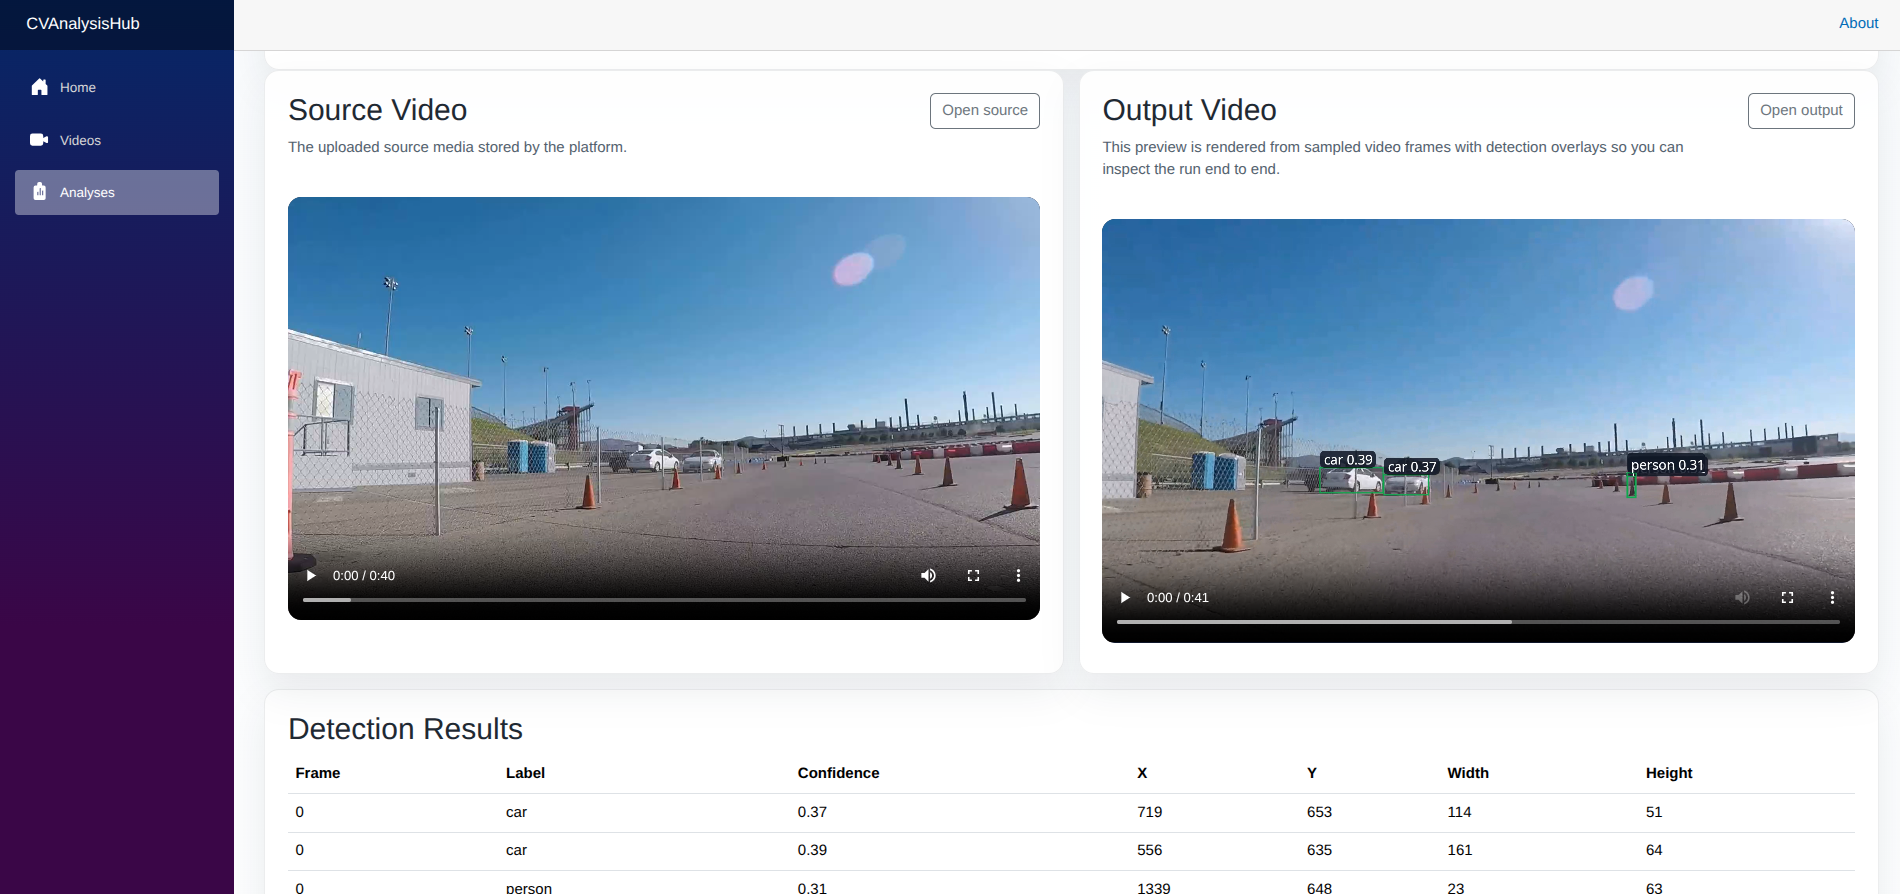
\includegraphics[width=0.95\textwidth,height=0.58\textheight,keepaspectratio]{figures/screenshots/blazor-analysis-details_2.png}
        \caption{Blazor интерфейс с таблица на отделните detection results за завършения анализ}
        \label{fig:blazor-analysis-details-results}
    \end{figure}
}{}

\IfFileExists{figures/screenshots/avalonia-analysis-details.png}{
    \begin{figure}[htbp]
        \centering
        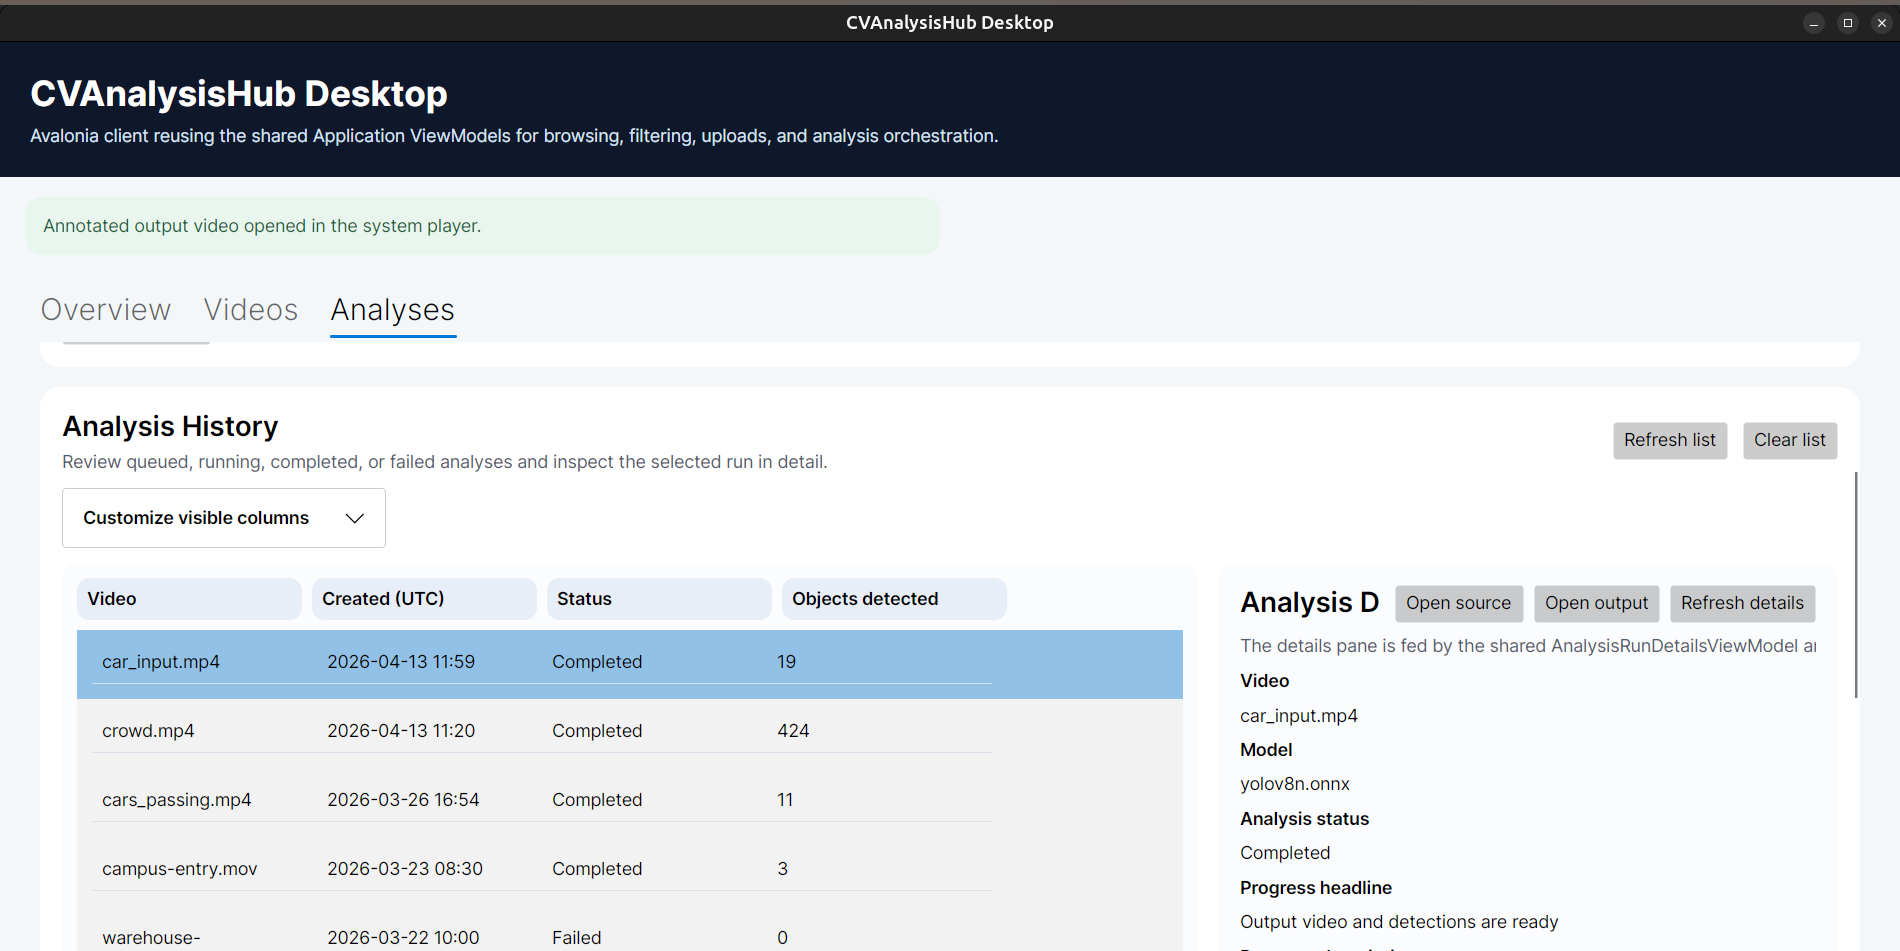
\includegraphics[width=0.95\textwidth,height=0.58\textheight,keepaspectratio]{figures/screenshots/avalonia-analysis-details.png}
        \caption{Avalonia интерфейс със същия завършен analysis run и синхронизирани резултати}
        \label{fig:avalonia-analysis-details}
    \end{figure}
}{}

\IfFileExists{figures/screenshots/reusable-filters-list.png}{
    \begin{figure}[htbp]
        \centering
        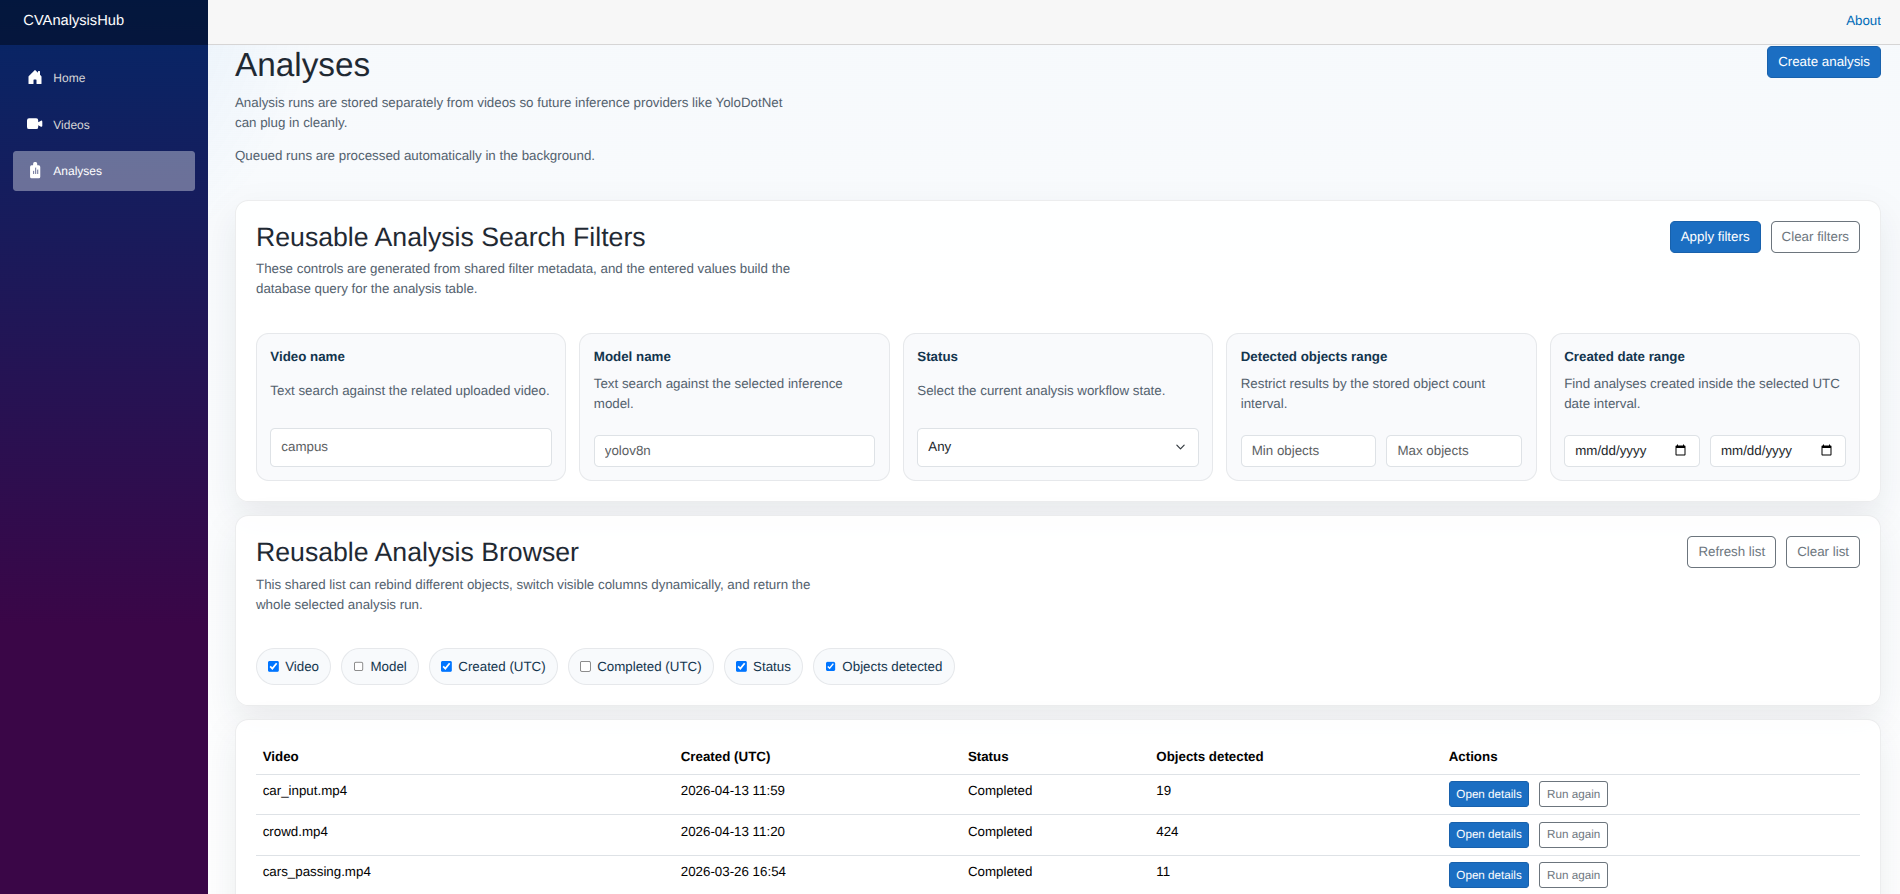
\includegraphics[width=0.95\textwidth,height=0.58\textheight,keepaspectratio]{figures/screenshots/reusable-filters-list.png}
        \caption{Демонстрация на преизползваемо филтриране и преизползваема визуализация на списък от обекти}
        \label{fig:reusable-filters-list}
    \end{figure}
}{}

\section{Демонстрация на преизползване}

Уеб клиентът показва преизползваемо филтриране върху два различни набора от данни. При \texttt{Videos} са реализирани филтри по име, статус, продължителност и дата на качване, а при \texttt{AnalysisRuns}, по видео, модел, статус, брой открити обекти и дата на създаване. Същественото е, че една и съща инфраструктура за филтриране работи върху различни модели без да бъде писана отново за всеки от тях.

Подобен ефект се наблюдава и при преизползваемата визуализация на списъци от обекти. Потребителят може да променя видимите колони, да избира конкретен ред и да работи с целия съответстващ обект, независимо каква част от него е визуализирана в таблицата. Тази функционалност е приложена както за \texttt{Videos}, така и за \texttt{AnalysisRuns}, което показва, че механизмът работи върху повече от един тип данни.

\chapter{Заключение}

В крайния си вид проектът представлява работещо .NET приложение, което покрива съществените изисквания на практическото задание и в същото време остава смислено от инженерна гледна точка. Системата използва MVVM, поддържа две различни View технологии, използва споделени ViewModel-и, работи с SQLite и PostgreSQL чрез общ модел и общ бизнес слой и включва преизползваеми функционалности за филтриране и визуализиране на списъци от обекти.

Най-важният архитектурен извод от разработката е, че правилното разделение по слоеве дава по-добър резултат от механично разпределение на файловете по шаблонни папки. Чрез такова разделение проектът постигна споделена приложна логика, технологично независими ViewModel-и, конфигурационно превключване между две СУБД и преизползваеми абстракции за потребителски интерфейс, без да жертва разбираемостта на реализацията.

От практическа гледна точка разработката показа и още нещо важно. За добър курсов проект не е достатъчно кодът да бъде архитектурно коректен. Необходимо е системата да бъде стабилна в реална среда, демонстрационно ясна и функционално завършена. Именно поради това в проекта беше обърнато внимание не само на модела и слоя за съхранение, но и на фоновата обработка, обработката на видео, синхронизацията между двата клиента и подобренията в Avalonia интерфейса.

Макар текущият вариант вече да е достатъчно завършен за целите на заданието, проектът има потенциал и за бъдещо развитие. Възможни посоки са по-богато визуализиране на резултатите, въвеждане на миграции вместо \texttt{EnsureCreated}, по-пълно изравняване на функционалността между двата клиента и допълнителни аналитични функции върху резултатите от детекцията.

\phantomsection
\addcontentsline{toc}{chapter}{Литература}

\small
\begin{thebibliography}{99}

\bibitem{assignment02}
Практически проект ПС/СПл 2026, \enquote{02 - Задание и Теми - Практически Проект ПС\_СПл 2026.pdf}, локален файл от курса.

\bibitem{assignment03}
Практически проект ПС/СПл 2026, \enquote{03 - Указания - Практически Проект ПС\_СПл 2026.pdf}, локален файл от курса.

\bibitem{assignment01}
Практически проект ПС/СПл 2026, \enquote{01 - Избор Теми - Практически Проект ПС\_СПл 2026.pdf}, локален файл от курса.

\bibitem{avalonia}
Avalonia UI documentation, \url{https://docs.avaloniaui.net/}

\bibitem{blazor}
Microsoft Learn, Blazor documentation, \url{https://learn.microsoft.com/aspnet/core/blazor/}

\bibitem{efcore}
Microsoft Learn, Entity Framework Core documentation, \url{https://learn.microsoft.com/ef/core/}

\bibitem{sqlite}
SQLite Documentation, \url{https://www.sqlite.org/docs.html}

\bibitem{postgresql}
PostgreSQL Documentation, \url{https://www.postgresql.org/docs/}

\bibitem{plantuml}
PlantUML official documentation, \url{https://plantuml.com/}

\bibitem{plantumllatex}
PlantUML LaTeX support, \url{https://plantuml.com/latex}

\bibitem{vscodeplantuml}
VSCode Marketplace, PlantUML extension by jebbs, \url{https://marketplace.visualstudio.com/items?itemName=jebbs.plantuml}

\bibitem{dbplantuml}
GitHub repository \texttt{chippyash/db-plantuml}, \url{https://github.com/chippyash/db-plantuml}

\bibitem{yolodotnet}
YoloDotNet repository / package documentation, \url{https://github.com/NickSwardh/YoloDotNet}

\bibitem{ultralyticsyolov8}
Ultralytics, \enquote{Introducing Ultralytics YOLOv8}, \url{https://www.ultralytics.com/blog/introducing-ultralytics-yolov8}

\bibitem{ultralyticsmodels}
Ultralytics YOLO model documentation and model comparison tables, \url{https://huggingface.co/Ultralytics/YOLOv8}

\bibitem{ffmpeg}
FFmpeg Documentation, \url{https://ffmpeg.org/documentation.html}

\end{thebibliography}


\end{document}
